%% 
%% Copyright 2007-2020 Elsevier Ltd
%% 
%% This file is part of the 'Elsarticle Bundle'.
%% ---------------------------------------------
%% 
%% It may be distributed under the conditions of the LaTeX Project Public
%% License, either version 1.2 of this license or (at your option) any
%% later version.  The latest version of this license is in
%%    http://www.latex-project.org/lppl.txt
%% and version 1.2 or later is part of all distributions of LaTeX
%% version 1999/12/01 or later.
%% 
%% The list of all files belonging to the 'Elsarticle Bundle' is
%% given in the file `manifest.txt'.
%% 

%% Template article for Elsevier's document class `elsarticle'
%% with numbered style bibliographic references
%% SP 2008/03/01
%%
%% 
%%
%% $Id: elsarticle-template-num.tex 190 2020-11-23 11:12:32Z rishi $
%%
%%
\documentclass[final,5p,times,twocolumn, 8pt, a4paper]{elsarticle}
% \usepackage[utf8]{vietnam}

%% Use the option review to obtain double line spacing
%% \documentclass[authoryear,preprint,review,12pt]{elsarticle}

%% Use the options 1p,twocolumn; 3p; 3p,twocolumn; 5p; or 5p,twocolumn
%% for a journal layout:
%% \documentclass[final,1p,times]{elsarticle}
%% \documentclass[final,1p,times,twocolumn]{elsarticle}
%% \documentclass[final,3p,times]{elsarticle}
%% \documentclass[final,3p,times,twocolumn]{elsarticle}
%% \documentclass[final,5p,times]{elsarticle}
%% \documentclass[final,5p,times,twocolumn]{elsarticle}

%% For including figures, graphicx.sty has been loaded in
%% elsarticle.cls. If you prefer to use the old commands
%% please give \usepackage{epsfig}

%% The amssymb package provides various useful mathematical symbols
\usepackage{amssymb}
\usepackage{enumitem}
\usepackage{color}
\usepackage[pdftex, % Sử dụng PDF TeX
bookmarks=true, % Tạo bookmarks trong tập tin PDF
colorlinks=false, % Chữ có màu
pdfencoding=auto, % Tự động điều chỉnh encoding của PDF
unicode=true, % Sử dụng Unicode
pdffitwindow=true, % Fit cho vừa cửa sổ
pdfstartview={FitW}, % Zoom file PDF cho vừa khít với nội dung
pdftoolbar=false, % Ẩn đi tool bar trong PDF viewer
pdfmenubar=false, % Ẩn đi menu bar trong PDF viewer
breaklinks=true % Tránh tràn dòng với liên kết
]{hyperref}
%% The amsthm package provides extended theorem environments
%% \usepackage{amsthm}

%% The lineno packages adds line numbers. Start line numbering with
%% \begin{linenumbers}, end it with \end{linenumbers}. Or switch it on
%% for the whole article with \linenumbers.
%% \usepackage{lineno}


\journal{HUST 2024 Graduation Ceremony}

\begin{document}

    \begin{frontmatter}

        %% Title, authors and addresses

        %% use the tnoteref command within \title for footnotes;
        %% use the tnotetext command for theassociated footnote;
        %% use the fnref command within \author or \address for footnotes;
        %% use the fntext command for theassociated footnote;
        %% use the corref command within \author for corresponding author footnotes;
        %% use the cortext command for theassociated footnote;
        %% use the ead command for the email address,
        %% and the form \ead[url] for the home page:
        %% \title{Title\tnoteref{label1}}
        %% \tnotetext[label1]{}
        %% \author{Name\corref{cor1}\fnref{label2}}
        %% \ead{email address}
        %% \ead[url]{home page}
        %% \fntext[label2]{}
        %% \cortext[cor1]{}
        %% \affiliation{organization={},
        %%             addressline={},
        %%             city={},
        %%             postcode={},
        %%             state={},
        %%             country={}}
        %% \fntext[label3]{}


        \title{Invitation to HUST 2024 Graduation Ceremony | English Version}

        \author[1]{Tien-Thanh Bui\corref{cor1}}

        \cortext[cor1]{Corresponding author}
        \ead{bu1th4nh.127@gmail.com}
        \ead[url]{https://github.com/bu1th4nh}




        \affiliation[1]{organization={Faculty of Mathematics and Informatics, Hanoi University of Science and Technology},
                    addressline={No. 1 Dai Co Viet},
                    city={Hai Ba Trung District, Hanoi},
                    % postcode={},
                    % state={},
                    country={Vietnam}}


        \begin{abstract}
            In this paper, an invitation to the graduation ceremony is presented. The event will take place at Hanoi University of Science and Technology on May 12, 2024. The detailed information about the time, location, contact information, and some additional recommendations are provided. 

        \end{abstract}

        \begin{keyword}
            Graduation \sep Hanoi University of Science and Technology \sep Bachelor of Science
        \end{keyword}

    \end{frontmatter}

    %% \linenumbers

    %% main text
    \section{Introduction}
        \par Graduation ceremony is an important event for every student. It marks the end of a chapter and the beginning of a new one. In this paper, an invitation to the graduation ceremony for Tien-Thanh Bui is presented. Section 1 provides the background information about the event. Section 2 presents the methodology and information used to construct the invitation. Section 3 concludes the paper.


    \section{Methodology}
        \par The invitation is constructed using LaTeX, with specific information edited and added for the author, including the location, time, schedule, and additional recommendations.

        \subsection{Time}
            \par The event will take place on \textcolor{red}{\textbf{May 12, 2024}}. The detailed schedule is as follows:
            \begin{enumerate}[label=\roman*)]
                \item From 09:30 to 13:00: Pre-party and photo-taking at the university campus with casual attire.
                \item From 13:00 to 14:00: Graduation ceremony at C2 Auditorium.
                \item From 14:00 to 17:30: Photo-taking at the university campus with graduation attire.
            \end{enumerate}

        \subsection{Place}
            \par The graduation ceremony will take place at \textcolor{red}{\textbf{Hanoi University of Science and Technology, No. 1 Dai Co Viet, Hai Ba Trung District}}. Figure \ref{fig:hust} shows the location marked on Google Earth. The area colored in \textcolor{red}{red}, with yellow border is the university campus, where the pre-party and photo-taking will be held. The marker in \textcolor{green}{green} indicates the C2 Auditorium, where the graduation ceremony will take place.
            \begin{figure}
                \centering
                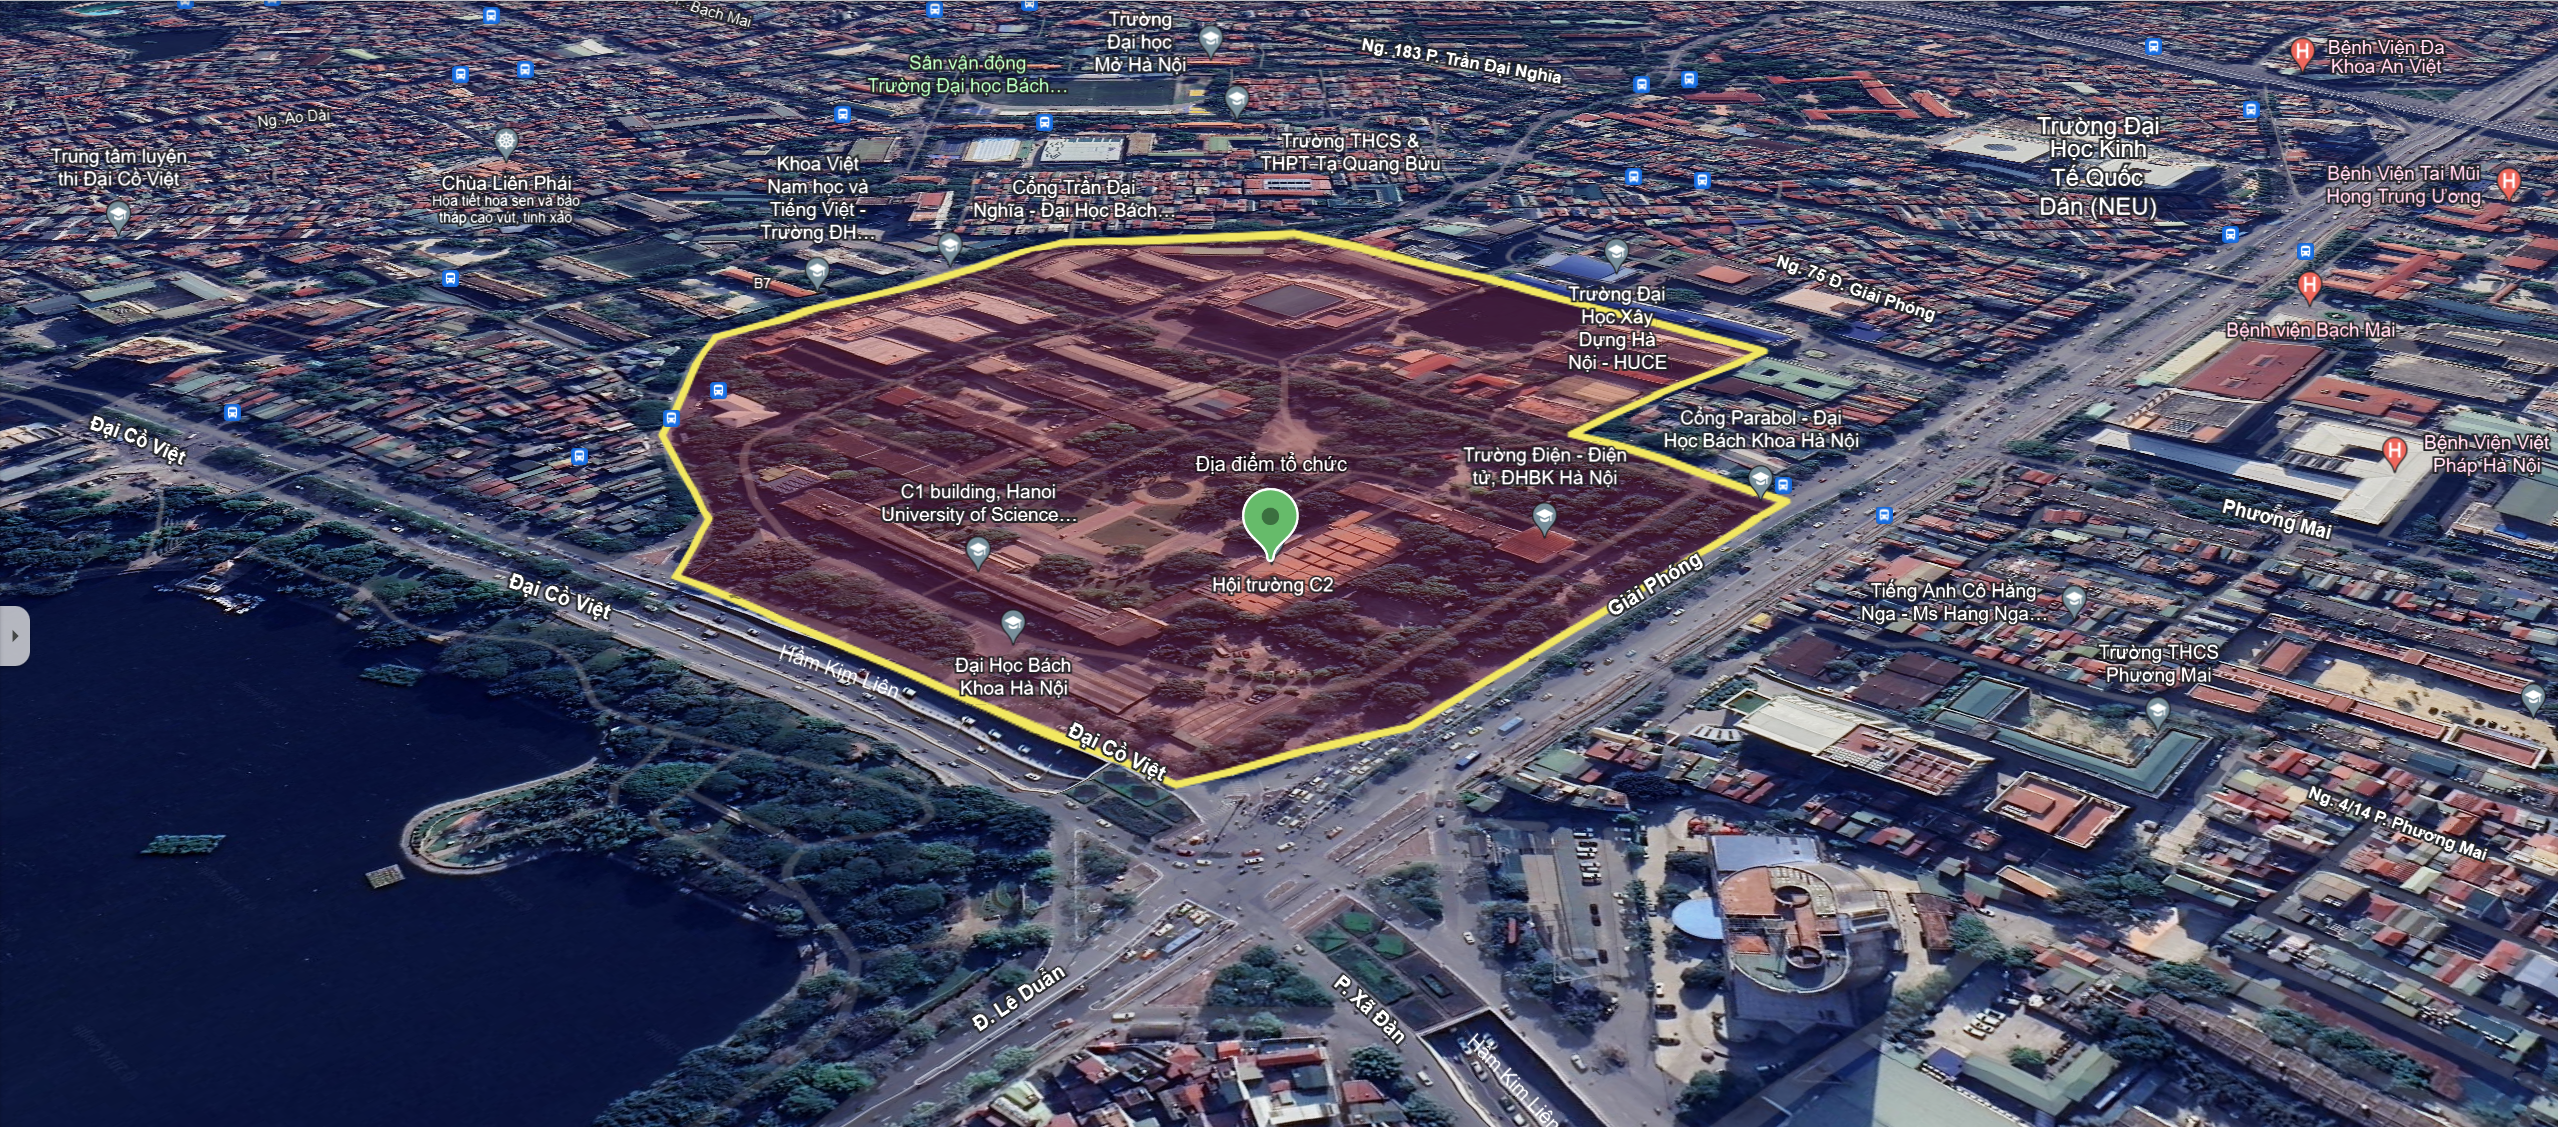
\includegraphics[width=0.45\textwidth]{place.png}
                \caption{Location on Google Earth.}
                \label{fig:hust}
            \end{figure}
            
        
        \subsection{Contact Information}
            \par To contact, please reach out via the following ways:
            \begin{itemize}
                \item \textbf{Facebook/Messenger}: \texttt{\href{https://www.facebook.com/bu1th4nh.127}{facebook.com/bu1th4nh.127}}
                \item \textbf{Phone number}: \texttt{\href{tel:0329436968}{0329436968}}
                \item \textbf{E-mail}: \texttt{\href{mailto:bu1th4nh.127@gmail.com}{bu1th4nh.127@gmail.com}}
            \end{itemize}


        \subsection{Some Recommendations}
            \par To prepare for the event, please note the following:
            \begin{itemize}
                \item Bring an umbrella as the weather on May 12 may be hot and rainy in the late afternoon,
                \item Bring water as everyone will get thirsty,
                \item Your presence is an honor and joy for the author.
            \end{itemize}

    \section{Conclusion}
        \par The event will take place on May 12, 2024 at Hanoi University of Science and Technology. All detailed information has been presented in this invitation. The author sincerely thanks and looks forward to the attendance of all friends and family.

        

\end{document}
\endinput
%%
%% End of file `elsarticle-template-num.tex'.
